\scanpage{81}
\mspage{72}
% archive sheet number: 81

\[
\begin{aligned}
 \Sigma_M&\longrightarrow\unsure{\mathcal{P}|P}(P)\\
 S&\longmapsto\unsure{\varphi|\phi}(S)\ (=|S|^{\circ})
\end{aligned}
\]
est injective, on trouve \unsure{un|une} inverse à gauche en associant, à toute partie $Q\deleted{\unsure{\subset}}$ de $P$, l'ens
\[
 \deleted{\unsure{S_Q=}}\quad\{X\in M\mid\varphi(X)\subset Q\}
\]
ou plutôt (comme celui-ci n'est peut-être pas lui-même un $\operatorname{supp}^{\circ}$)
\[
 S_Q=\operatorname{supp}^{\circ}(\{X\in M\mid\varphi(X)\subset Q\}).
\]

Est-on déraisonnable, d'espérer que le plongement précédent commute $\unsure{\rightleftarrows|\complement}$, i.e. qu'on puisse y comprendre quelque chose aux supports\inserted{intrinsèques} des figures (élémentaires en l'occurrence) qui ne soit \deleted{pas} ni compatible, ni ne le devienne après subdivisions.
% margin note written slanted
\margin{Il ne commute pas aux $A\cap B$ déjà dans le cas de la \unsure{réalis.} tautologique \unsure{d'un|d'une} \unsure{cadre|corde} topologique pour les supports associés à deux ``cellules'', cf \unsure{figure}.}
% Drawing in the left margin, below the slanted note.
\figure{
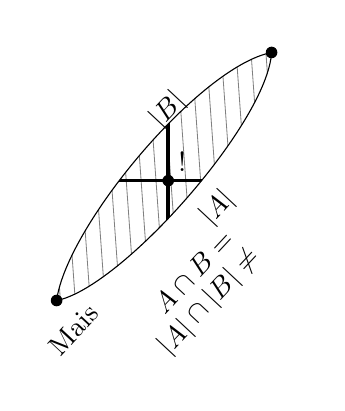
\begin{tikzpicture}[scale=1.05]
\path[use as bounding box] (-.35,-1.0) rectangle (3.15,3.3);
\begin{scope}
\clip (0,0) .. controls (.12,.9) and (1.73,2.83) .. (2.6,3.0) .. controls (2.55,2.15) and (.78,.15) .. (0,0);
\foreach \x in {-0.3,-0.12,0.06,0.24,0.42,0.60,0.78,0.96,1.14,1.32,1.50,1.68,1.86,2.04,2.22,2.40,2.58,2.76}{\draw[gray,line width=.3pt] (\x,-.2)--(\x-.25,3.3);}
\draw[line width=1.3pt] (.7,1.45)--(1.95,1.45);
\draw[line width=1.3pt] (1.35,.75)--(1.35,2.2);
\end{scope}
\draw (0,0) .. controls (.12,.9) and (1.73,2.83) .. (2.6,3.0) .. controls (2.55,2.15) and (.78,.15) .. (0,0);
\fill (0,0) circle (2pt) (2.6,3.0) circle (2pt) (1.35,1.45) circle (2pt);
\node at (1.52,1.68) {!};
\node[rotate=47] at (1.35,2.3) {$|B|$};
\node[rotate=47] at (1.95,1.12) {$|A|$};
\node[rotate=47] at (.2,-.35) {\deleted{\unsure{Mais}}};
\node[rotate=47] at (1.65,.35) {$A\cap B=\varnothing$};
\node[rotate=47] at (1.85,-.02) {$|A|\cap|B|\ne\varnothing$};
\end{tikzpicture}}

Aussi faudrait-il à présent que je me limite à des supports de nature très particulière, \unsure{attachés} à une figure (supports ``constructibles'')
